
%(BEGIN_QUESTION)
% Copyright 2010, Tony R. Kuphaldt, released under the Creative Commons Attribution License (v 1.0)
% This means you may do almost anything with this work of mine, so long as you give me proper credit

Consider this control system, set up to maintain the temperature of a chemical reactor vessel at a constant (``setpoint'') value.  The reactor's source of heat is a steam ``jacket'' where hot steam is admitted through a motor-operated (M) control valve (TV) according to the temperature inside the reactor sensed by the temperature transmitter (TT):

$$\includegraphics[width=15.5cm]{i00137x01.eps}$$

You arrive at work one day to find the operator very upset.  The last batch of product emptied from the reactor was out of spec, as though the temperature were too cold, yet the controller (TIC) displays the temperature to be right at setpoint where it should be: 175 $^{o}$F.

Your first step is to go to the reactor and look at the temperature indicating gauge (TI) mounted near the same point as the temperature transmitter.  It registers a temperature of only 137 $^{o}$F.

From this information, determine what is the most likely source of the problem, and explain how you made that determination.

\vskip 20pt \vbox{\hrule \hbox{\strut \vrule{} {\bf Suggestions for Socratic discussion} \vrule} \hrule}

\begin{itemize}
\item{} Why was it a good decision to consult the temperature gauge (TI) on the reactor as a first diagnostic step?
\item{} Suppose a fellow instrument technician were to suggest to you that the problem in this system could be a controller configured for the wrong action (e.g. direct action instead of reverse action).  Do you think this is a plausible explanation for the symptoms reported here?  Why or why not?
\item{} Could the problem be that someone left the controller in {\it manual} mode rather than automatic mode as it should be?  Explain why or why not.
\item{} Based on the P\&ID shown, are the instruments pneumatic or electronic?
\item{} Given the fact that we know this reactor is steam-heated, is it possible to conclude that the chemical reaction taking place inside it is either endothermic (heat-absorbing) or exothermic (heat-releasing)?
\item{} Safety shutdown systems often use a ``two-out-of-three'' (2oo3) voting algorithm to select the best measurement from three redundant transmitters.  Explain how this same concept may be applied by the instrument technician in the course of troubleshooting the problem.
\end{itemize}

\underbar{file i00137}
%(END_QUESTION)





%(BEGIN_ANSWER)

%(END_ANSWER)





%(BEGIN_NOTES)

The problem most likely lies with the temperature transmitter (TT).

\vskip 10pt

An important diagnostic principle here is that of a {\it two-out-of-three} vote.  By comparing three sources of information on the same variable and determining the majority agreement, we are able to better discern the actual value of that variable despite faults in the equipment.  The technician must determine which instrument is faulted based on a comparison of three points of data: two instruments (indicating controller and gauge) and the operator's assessment of the product batch.  Since two out of these three data sources agree (batch quality and temperature gauge), the most likely fault is in the temperature transmitter/indicating controller loop.

An alternative possibility to the transmitter being bad is a mis-calibration of the controller's process variable input, causing it to register falsely high even if it receives the correct milliamp signal from the transmitter.  Another possibility is the primary sensing element (RTD, thermocouple, etc.) being faulty, sending the transmitter an incorrect signal.






\vskip 20pt \vbox{\hrule \hbox{\strut \vrule{} {\bf Virtual Troubleshooting} \vrule} \hrule}

This question is a good candidate for a ``Virtual Troubleshooting'' exercise.  Presenting the diagram to students, you first imagine in your own mind a particular fault in the system.  Then, you present one or more symptoms of that fault (something noticeable by an operator or other user of the system).  Students then propose various diagnostic tests to perform on this system to identify the nature and location of the fault, as though they were technicians trying to troubleshoot the problem.  Your job is to tell them what the result(s) would be for each of the proposed diagnostic tests, documenting those results where all the students can see.

During and after the exercise, it is good to ask students follow-up questions such as:

\begin{itemize}
\item{} What does the result of the last diagnostic test tell you about the fault?
\item{} Suppose the results of the last diagnostic test were different.  What then would that result tell you about the fault?
\item{} Is the last diagnostic test the best one we could do?
\item{} What would be the ideal order of tests, to diagnose the problem in as few steps as possible?
\end{itemize}

%INDEX% Basics, control loop troubleshooting: determining cause of control problem
%INDEX% Process: steam-heated reactor vessel (generic)

%(END_NOTES)


